\begin{mydef}
	Un rectangle est un quadrilatère qui possède \kw{quatre angles droits}.
\end{mydef}

\begin{myprops}
	\textbf{Si} un quadrilatère est un rectangle \textbf{alors} 
	\begin{itemize}
		\item il a \kw{quatre angles droits};
		\item ses \kw{diagonales} ont la \kw{même longueur}.
	\end{itemize}
\end{myprops}

\begin{myex}
	\begin{center}
		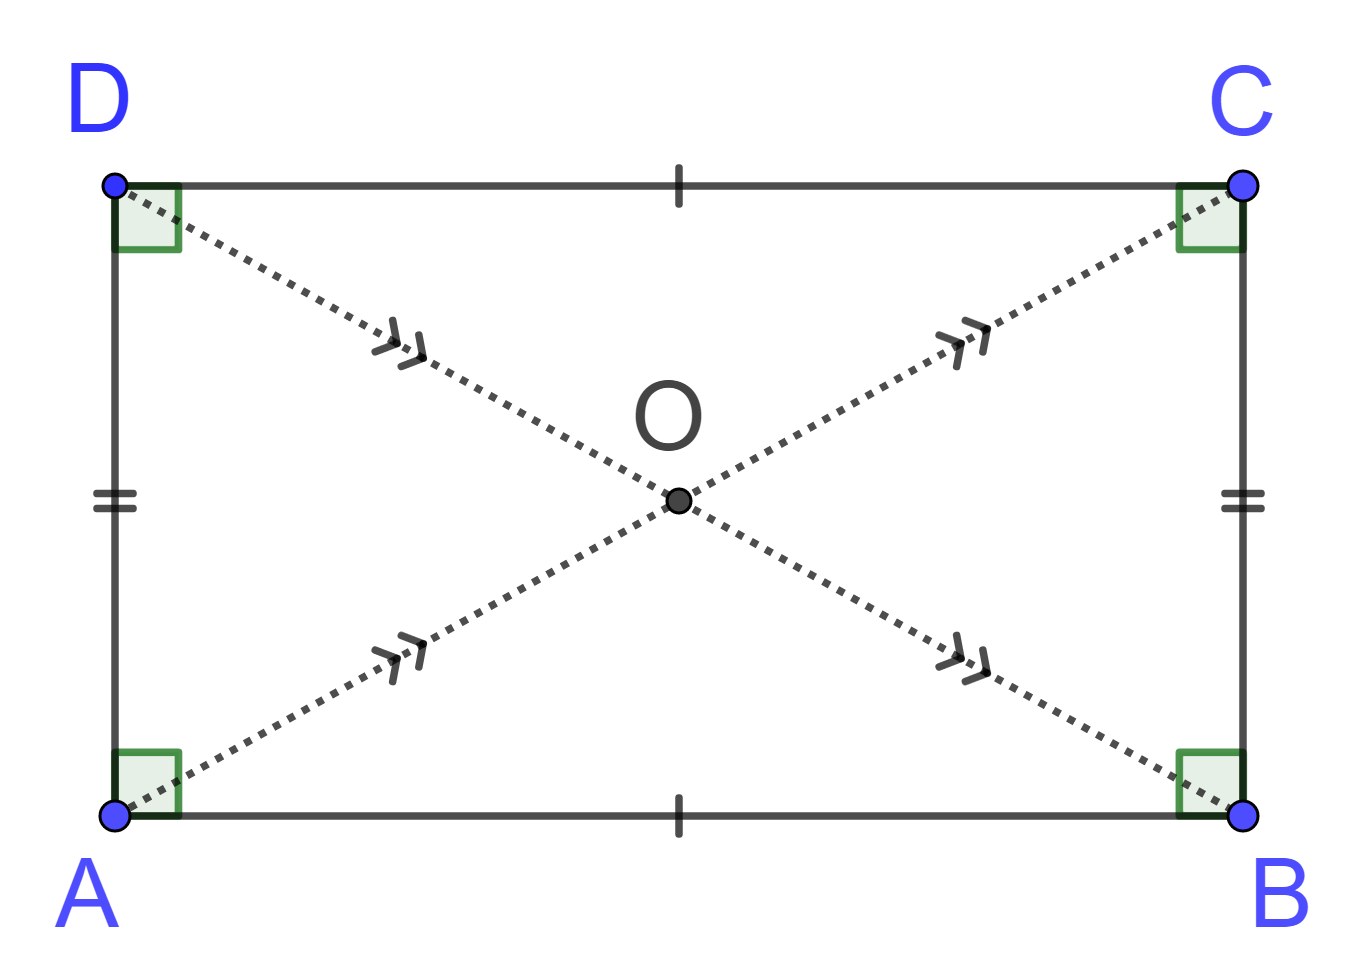
\includegraphics[scale=0.15]{rectangle}
	\end{center}

	ABCD est un rectangle donc :
		\begin{itemize}
			\item $\widehat{ABC} = \widehat{BCD} = \widehat{CDA} = \widehat{DAB} = 90\degree$;
			\item $AC = BD$.
		\end{itemize} 
\end{myex}